
\subsection{Graph reminder}

\subsubsection{Definitions}

A \textbf{directed} graph is tuple (V, E) where V is the set of vertices (also
called nodes) and $E \in V x V$ is the set of edges (also called arcs).\newline

A \textbf{path} is a suite of distinct nodes $n_0, n_1, ... n_(k-1)$ with $(n_i, n_(i+1))$ an
edge for all $0 \leq i \le k-1$. Node $n_0$ is the origin and node $n_(k-1)$ is the
destination.\newline

A \textbf{cycle} is suite of distinct nodes  $n_0, n_1, ... n_(k-1)$ with $(n_i, n_(i+1)\% k)$ an edge for all $0 \leq i \le k$.

\subsubsection{Graph representation}

A graph (directed or not)can be represented in many way such as an adjacency list or an adjacency matrix (matrix are not always the best as they don't take sparsity into account).

\begin{figure}[!ht]
    \centering
    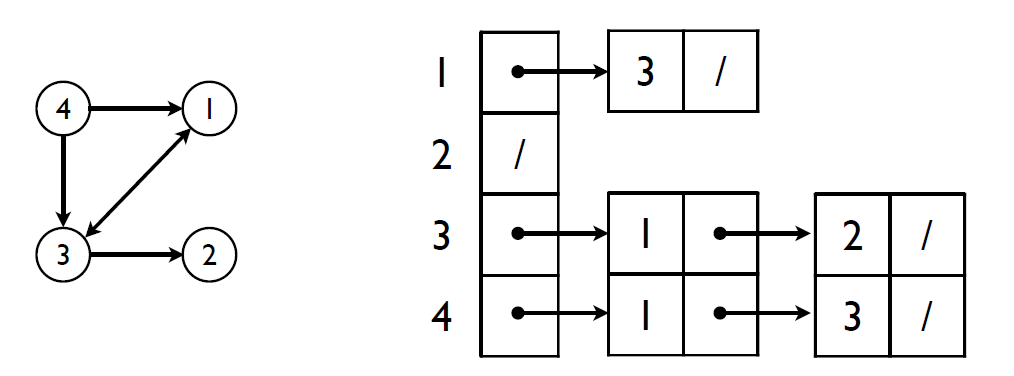
\includegraphics[width=0.3\linewidth]{AdjacencyList.png}
    \caption{Adjacency List example}
    \label{fig:AdjacencyList_example}
\end{figure}
\FloatBarrier

\subsubsection{DFS}

TODO ! \newline

Say that as we are in a graph, we need to color node that we have already explored so that we don't reexplore them. For the rest, everybody can do a dfs i guess.\newline

Complexity = O(nbNodes + nbEdges)\newline
As we have to check every edges at every node but we pass on each node once.

\subsection{Max flow}

Can be solved in polynomial time !

\subsubsection{Definitions}

s is the source \newline

t is the sink \newline

The \textbf{capacity} between two nodes a and b is denoted as c(a,b).
This value is positive if (a, b) is an edge of the graph, 0 if (a, b) is
not an edge.\newline

A \textbf{flow} is a vector f such that each composant is associated to a
pair of nodes. We denote by f(a,b) the flow quantity between
nodes a and b. We have following relation:

$$f(a,b) = -f(a,b)$$ 

An \textbf{instance of the Max Flow problem} is characterized by the
graph G = (V, E), the source s, the sink t and the vector of
capacity c.

\begin{figure}[!ht]
    \centering
    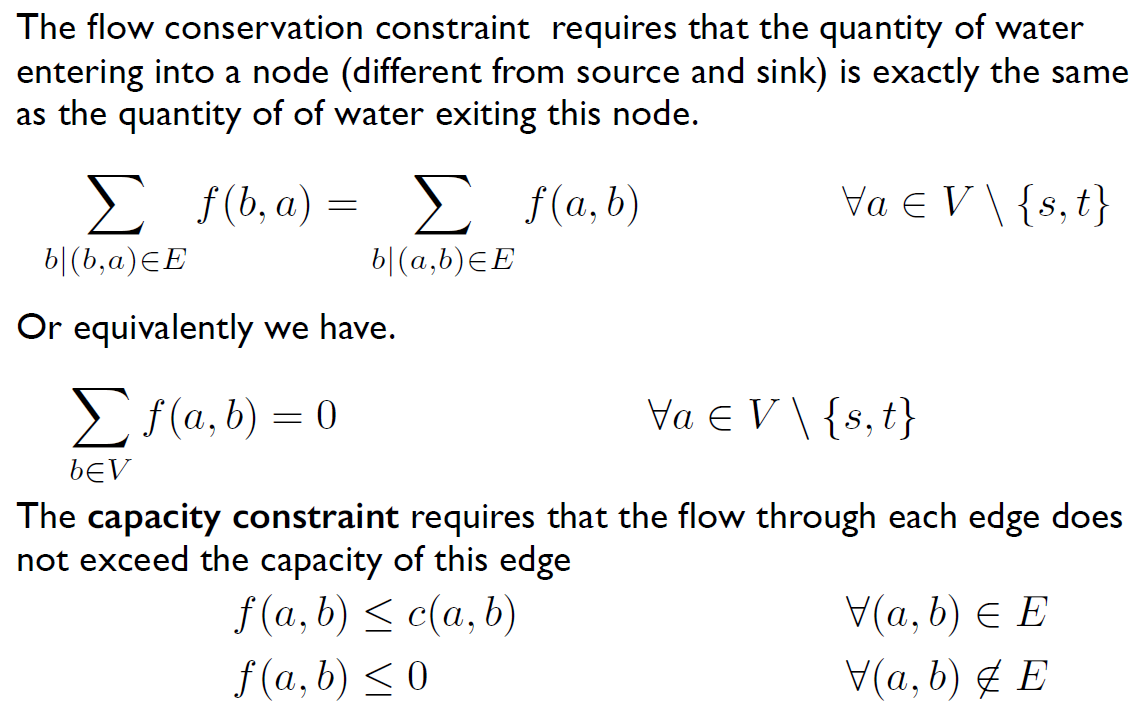
\includegraphics[width=0.7\linewidth]{MaxFlow2.png}
\end{figure}
\FloatBarrier

\begin{figure}[!ht]
    \centering
    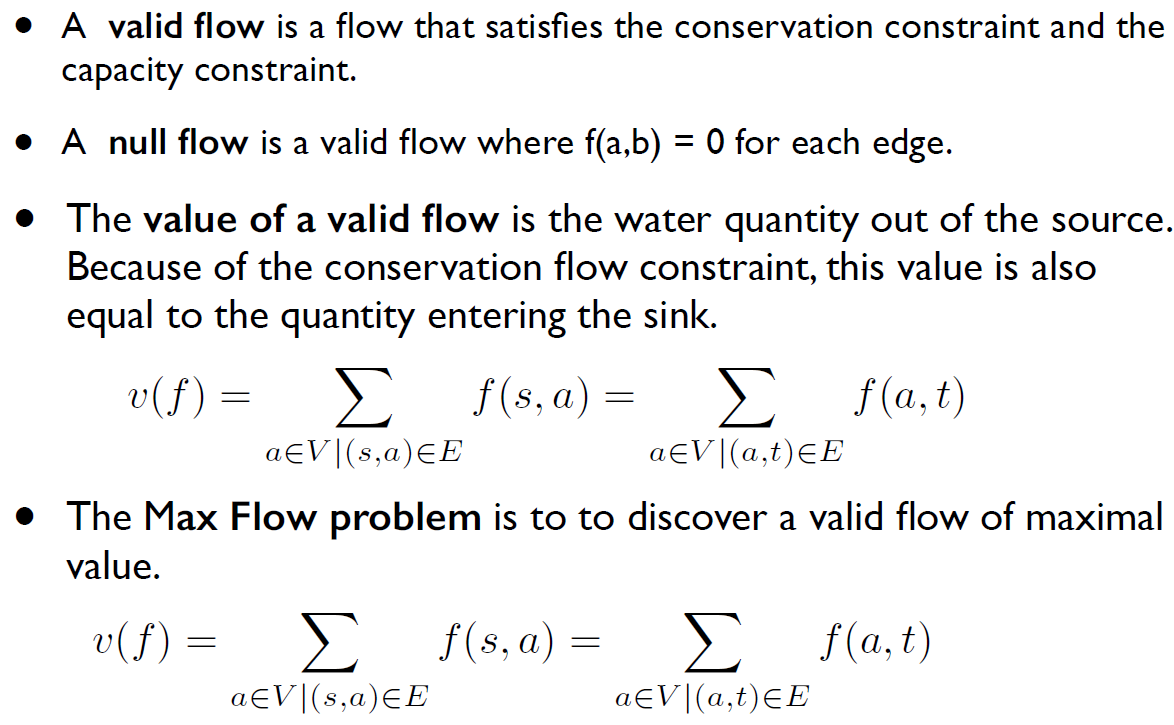
\includegraphics[width=0.7\linewidth]{MaxFlow1.png}
\end{figure}
\FloatBarrier

\textbf{Residual graph}Ø Gf = (V, Ef) are used to discover paths from the
source to the sink on which it is possible to push an
additional quantity of water and so increase the value of the
flow. This graph is composed of exactly the same nodes as the
original graph G = (V, E) but the edges may have a different
direction and a different (residual) capacity.

Basically if an edge is present only if it didn't reach it's maximal capacity and 
the residual capacity is is given by the quantity of the flow that can be added 
without violating the capacity of the edge.

A path joining the source s to the sink t in the residual graph Gf is
called \textbf{augmenting path}

\subsubsection{Graphical representation}

\begin{figure}[!ht]
    \centering
    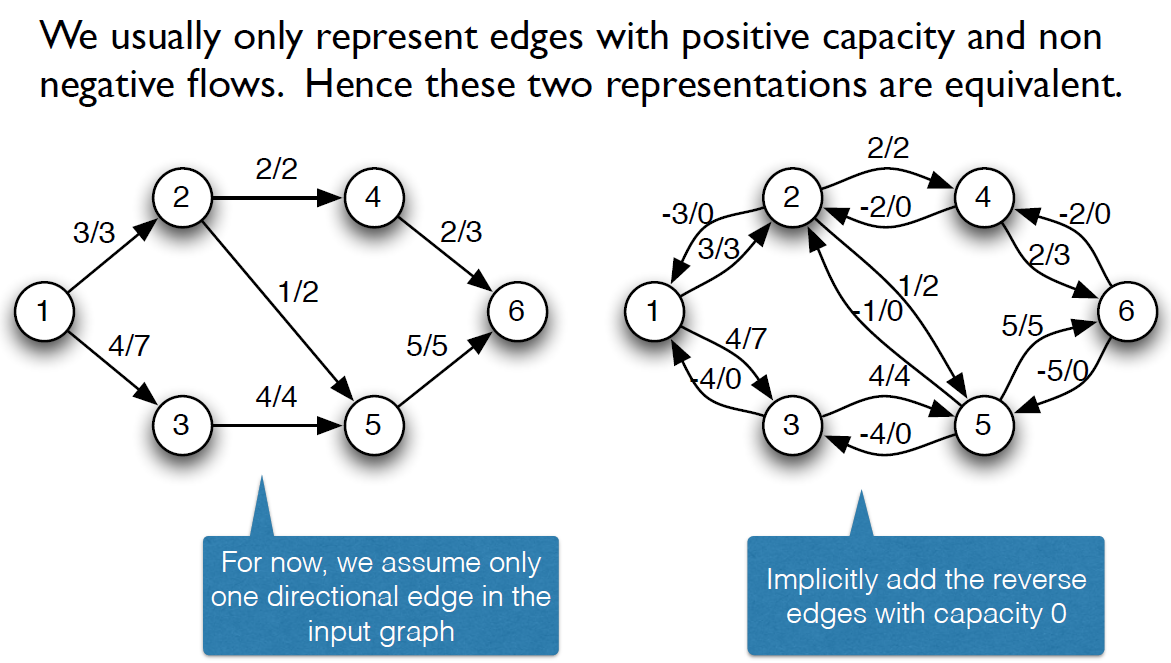
\includegraphics[width=0.7\linewidth]{MaxFlowGraphRepr.png}
\end{figure}
\FloatBarrier

For bidirectional edges, the reverse edge that we have will have the capacity of the second edge as shown in the example below.

\begin{figure}[!ht]
    \centering
    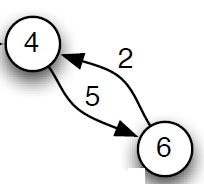
\includegraphics[width=0.7\linewidth]{MaxFlowBidirectionnalRepresentation.png}
\end{figure}
\FloatBarrier

\subsubsection{Ford-Fulkerson Algorithm}

\begin{figure}[!ht]
    \centering
    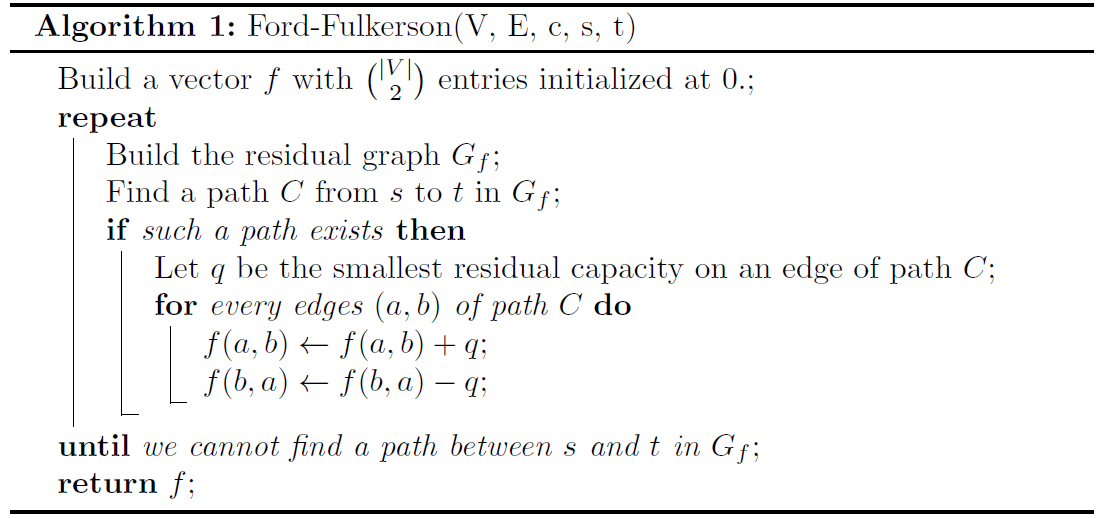
\includegraphics[width=0.9\linewidth]{MaxFlowAlgo.png}
\end{figure}
\FloatBarrier

Note : As is, the complexity of the algorithm is O(|V||E|U) with U the maximum flow of the graph. The complexity is thus not polynomial but pseudo-polynomial. For this algorithm to be polynomial you must use delta scaling. \newline

Delta scaling pseudocode :

\begin{lstlisting}
delta = X > 1
while true {
	Filter out all edges with capa < X in residual graph
	if you find an augmenting path :
		delta *= 2
		q = smallest capa of path
		for every edge of path do:
			f(a,b) = f(a,b) + q
			f(b,a) = f(b,a) - q
	else if delta > 1 :
		delta /= 2
	else
		break;
}
return result
\end{lstlisting}

As their are a maximum of log(U) iteration with delta scaling, the algorithm is of polynomial complexity. The complexity becomes O(|E|² log U)

\begin{figure}[!ht]
    \centering
    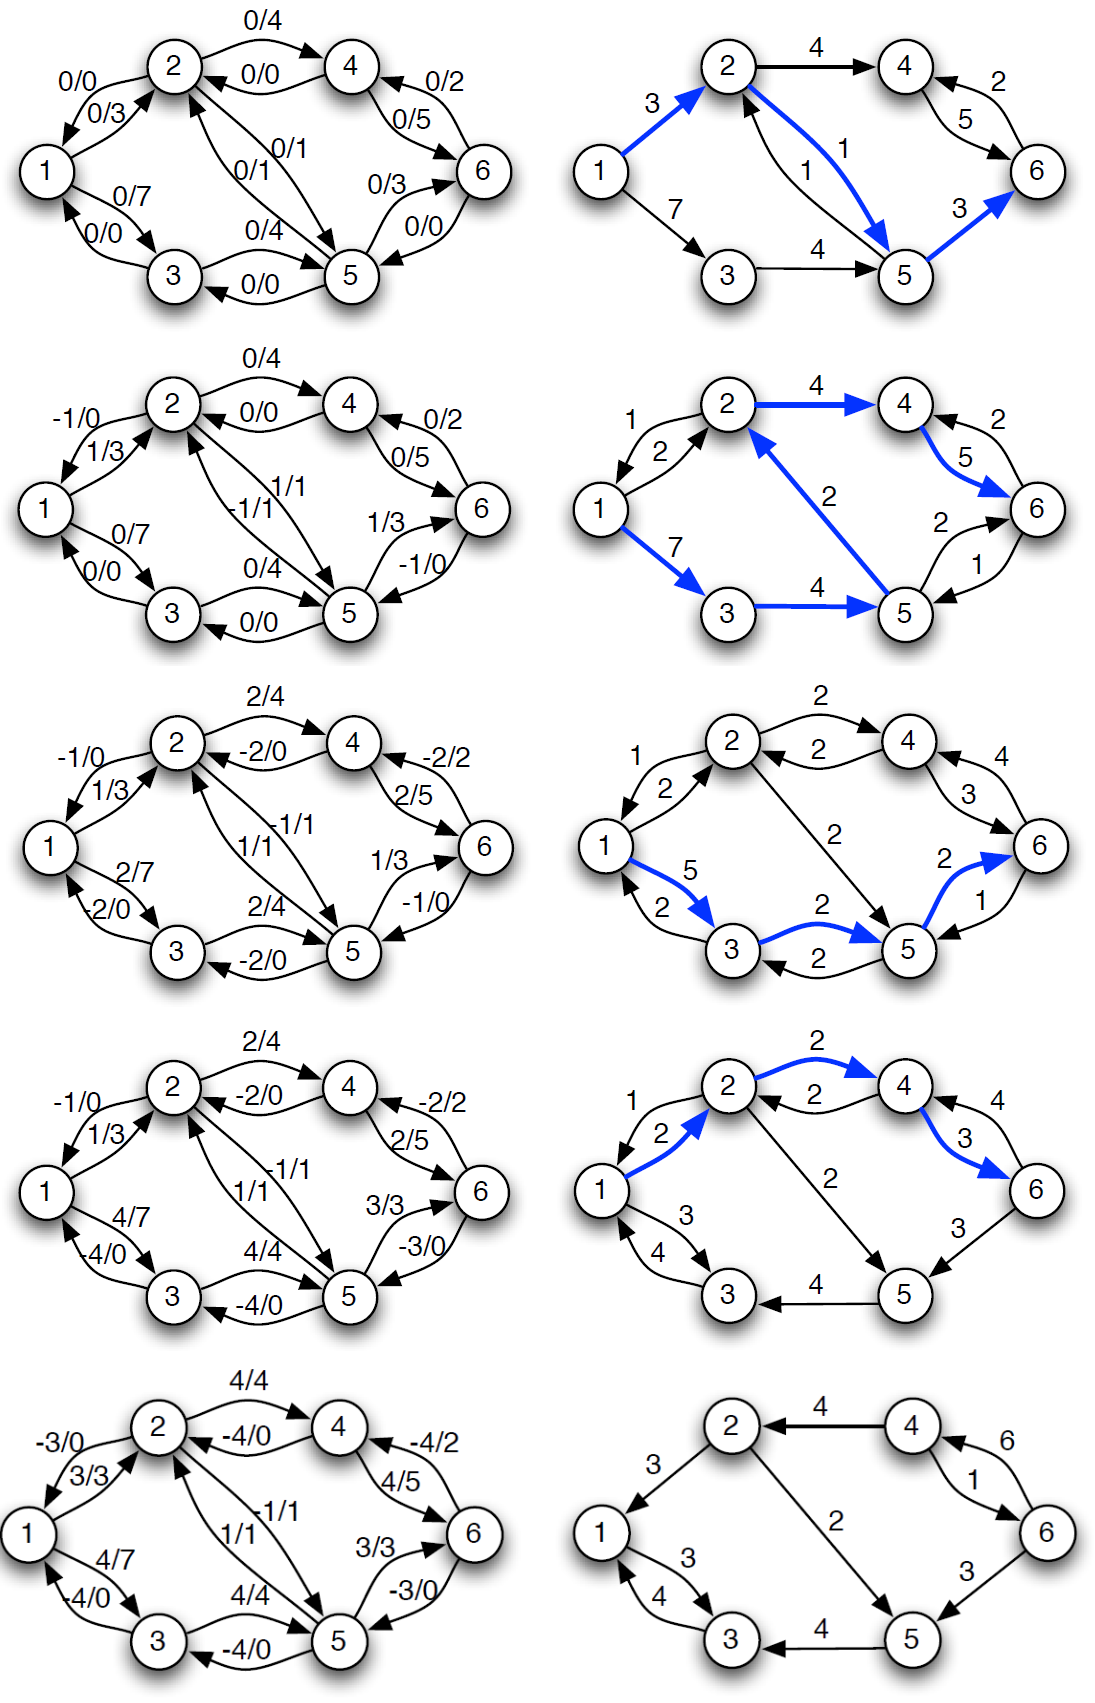
\includegraphics[width=0.55\linewidth]{MaxFlowAlgoExecutionExample.png}
    \caption{Ford-Fulkerson runtime example}
    \label{fig:Ford-Fulkerson_example}
\end{figure}

\subsubsection{Min flow}

\begin{figure}[!ht]
    \centering
    \includegraphics[width=0.7\linewidth]{MinFlow.png}
\end{figure}

Be careful that in some problem negative weight may be used and infinite loop must thus be avoided. => Use the Moore-Bellman-Ford algorithm \url{https://en.wikipedia.org/wiki/Bellman%E2%80%93Ford_algorithm} 

\subsection{Min cut}

How much cut do we have to make to partition a graph such that two node s and t, are in different partition. Answer == MaxFlow(s,t)

\subsubsection{Definitions}

\begin{figure}[!ht]
    \centering
    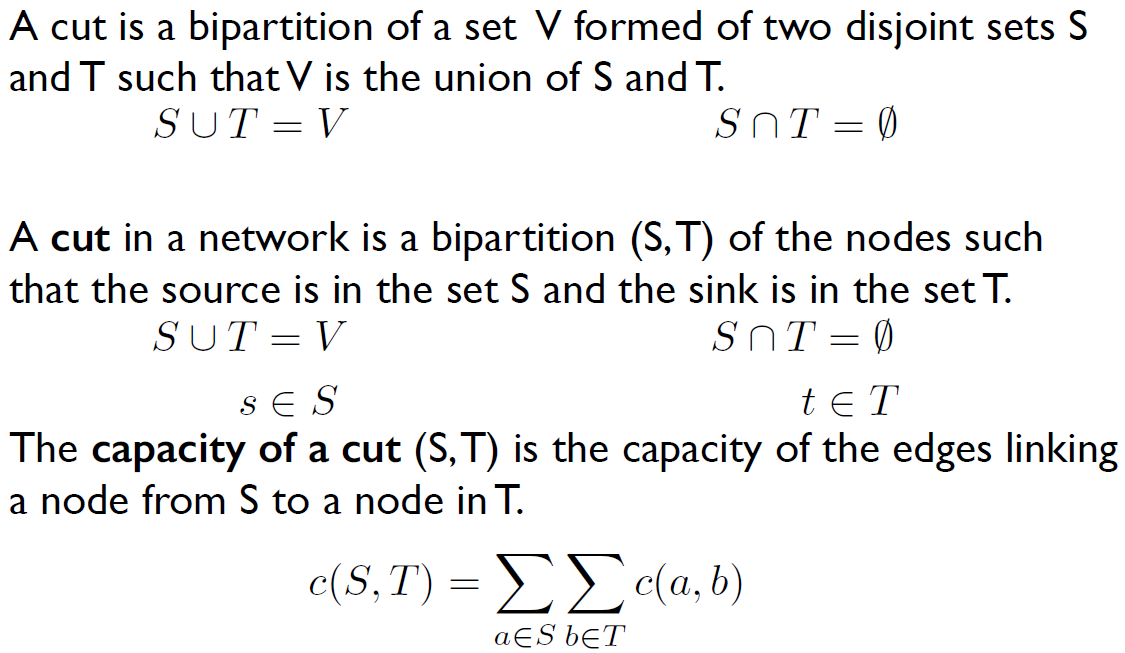
\includegraphics[width=0.7\linewidth]{CutDefinition.png}
\end{figure}
\FloatBarrier

\begin{figure}[!ht]
    \centering
    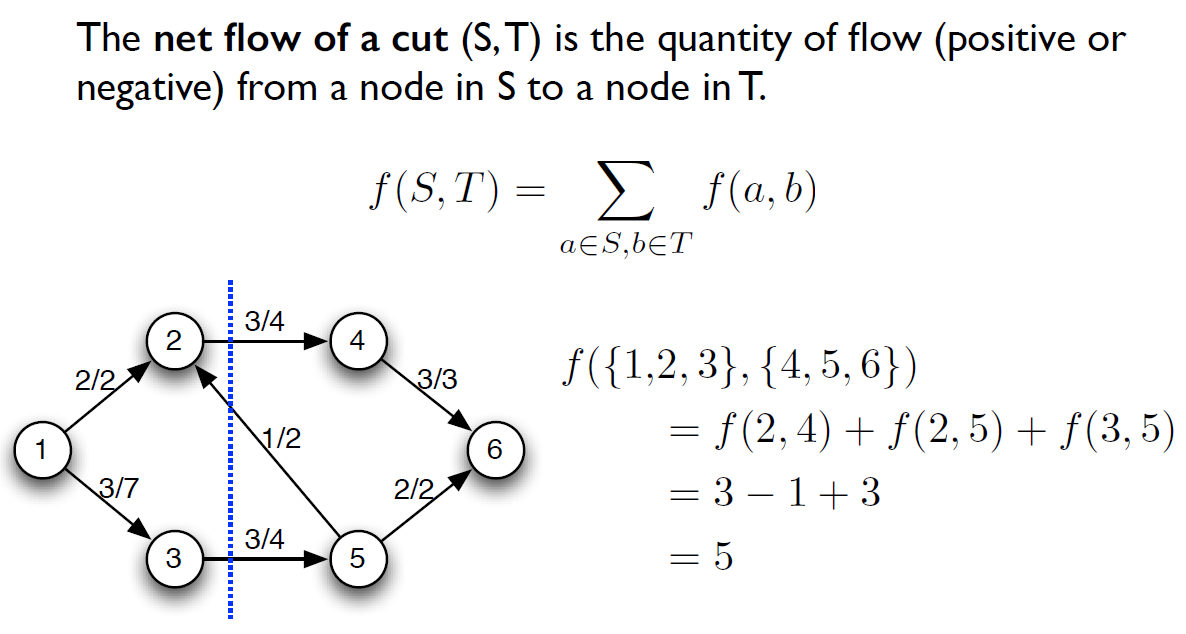
\includegraphics[width=0.7\linewidth]{CutDefinition1.png}
\end{figure}
\FloatBarrier

\subsubsection{Proof that min cut is solved by max flow}

\begin{figure}[!ht]
    \centering
    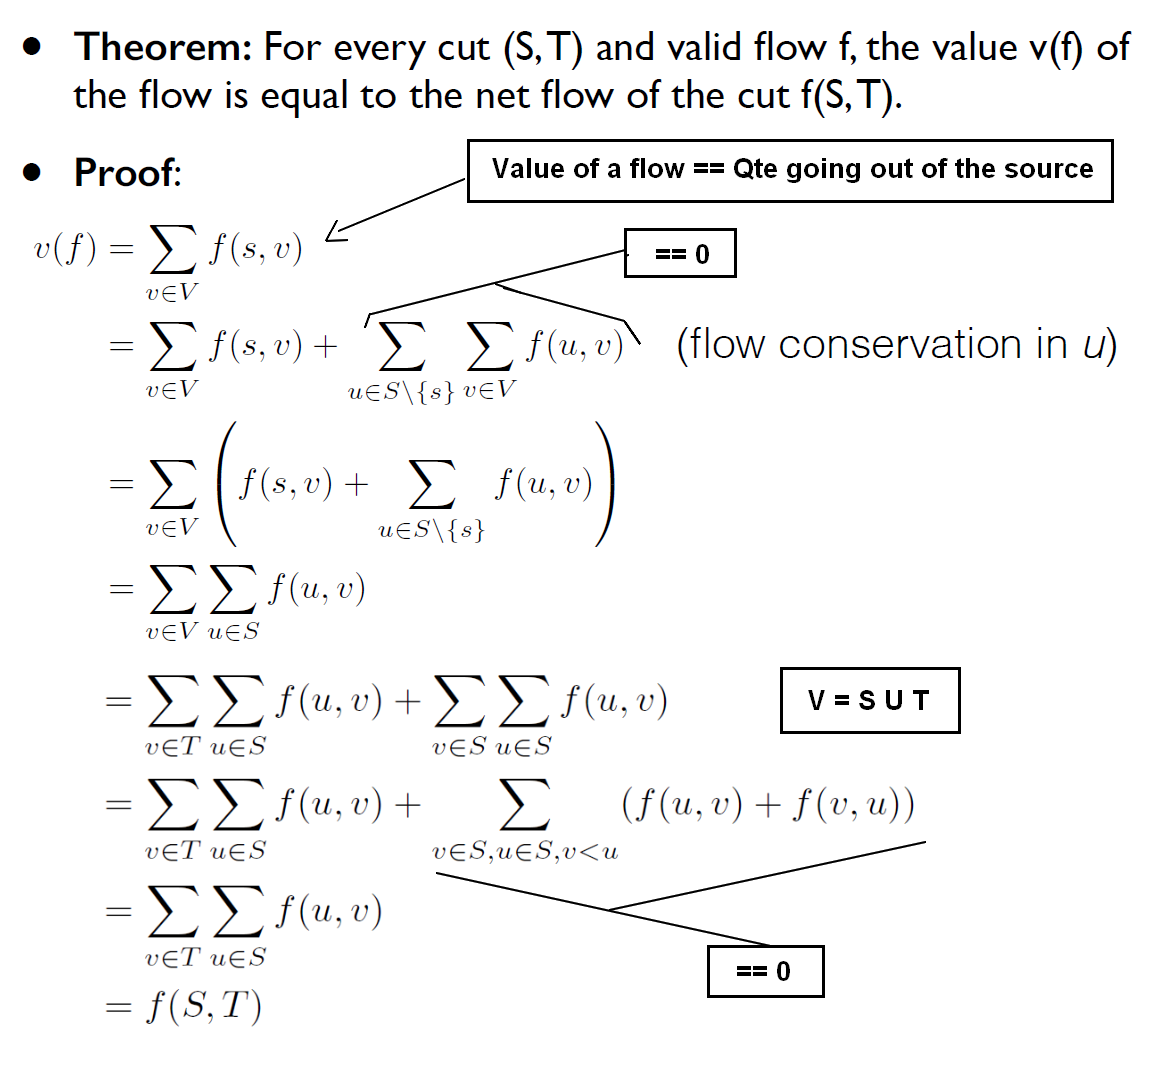
\includegraphics[width=0.7\linewidth]{CutProof.png}
\end{figure}
\FloatBarrier